\classicsectiondivider{From multimodal pretraining to Vietnamese AVSR.}

\subsection{AV-HuBERT Pretraining Pipeline}

\begin{frame}{Overview}
  \centering
  \vspace{-0.12cm}
  \begin{tikzpicture}[
    x=1cm,
    y=1cm,
    flow/.style={draw=ClassicNavy,thick,rounded corners=2pt,fill=ClassicSoft,
      align=center,minimum height=0.62cm,font=\scriptsize,inner sep=3pt},
    encoder/.style={flow,fill=HCMUTLightBlue!14},
    fusion/.style={flow,fill=green!12!white},
    target/.style={flow,fill=orange!16!white},
    loss/.style={flow,draw=red!70!black,fill=red!7!white},
    arrow/.style={-{Latex[length=2.1mm,width=1.4mm]},line width=0.65pt,draw=gray!80!black}
  ]
    % Input timelines
    \node[inner sep=0pt] (visual) at (-3.0,0.55)
      {
\includegraphics[width=4.55cm,height=0.60cm,keepaspectratio]{masked-visual-red.png}};
    \node[font=\tiny,below=0.02cm of visual] {Visual: $v_{1:T}\xrightarrow{M_v}\widetilde v_{1:T}$};
    \node[inner sep=0pt] (audio) at (3.0,0.55)
      {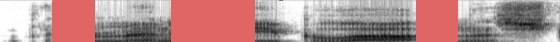
\includegraphics[width=4.55cm,height=0.60cm,keepaspectratio]{avhubert-audio-timesteps.png}};
    \node[font=\tiny,below=0.02cm of audio] {Audio: $a_{1:T}\xrightarrow{M_a}\widetilde a_{1:T}$};

    % Encoders and fused contextual representation
    \node[encoder,text width=3.25cm] (venc) at (-3.0,1.65)
      {\textbf{Visual encoder (ResNet-18)}\\[-0.05cm]$f_t^v=E_v(\widetilde v_t)$};
    \node[encoder,text width=3.25cm] (aenc) at (3.0,1.65)
      {\textbf{Audio encoder (Linear)}\\[-0.05cm]$f_t^a=E_a(\widetilde a_t)$};
    \node[fusion,text width=4.15cm] (fusion) at (0,2.85)
      {\textbf{Frame-wise fusion + modality dropout}\\[-0.05cm]
       $x_t=D_m\!\left([f_t^a;f_t^v]\right)$};
    \node[flow,text width=4.15cm,fill=ClassicBlue!11!white] (transformer) at (0,4.00)
      {\textbf{Transformer context encoder}\\[-0.05cm]
       $h_{1:T}=\operatorname{Transformer}(x_{1:T})$};
    \node[flow,text width=2.75cm] (prediction) at (-2.45,5.15)
      {\textbf{Cluster prediction}\\[-0.05cm]
       $p_t=\operatorname{Softmax}(Wh_t+b)$};

    % Pseudo-label branch
    \node[target,text width=1.85cm] (features) at (0.25,5.15)
      {MFCC / previous iteration\\[-0.05cm]$r_t^{(k-1)}$};
    \node[target,text width=1.35cm] (kmeans) at (2.55,5.15)
      {\textbf{K-means}};
    \node[target,text width=1.28cm] (targets) at (4.50,5.15)
      {Target IDs\\[-0.05cm]$z_t^{(k)}$};
    \node[loss,text width=4.35cm] (objective) at (0.85,6.30)
      {\textbf{Masked prediction objective}\\[-0.04cm]
       $\mathcal L_{\mathrm{pre}}=-\sum_{t\in M_a\cup M_v}\log p_t(z_t)$};

    % Main model path
    \draw[arrow] (visual.north) -- (venc.south);
    \draw[arrow] (audio.north) -- (aenc.south);
    \draw[arrow] (venc.north) -- (fusion.south west);
    \draw[arrow] (aenc.north) -- (fusion.south east);
    \draw[arrow] (fusion.north) -- (transformer.south);
    \draw[arrow] (transformer.north) -- (prediction.south);

    % Target and loss paths
    \draw[arrow] (features.east) -- (kmeans.west);
    \draw[arrow] (kmeans.east) -- (targets.west);
    \draw[arrow] (prediction.north) -- (objective.south west);
    \draw[arrow] (targets.north) -- (objective.south east);

  \end{tikzpicture}

  \note{[Sources] AV-HuBERT.pdf, Sections 3.2--3.4 and Equations 1--4; Weining Hsu, AAAI 2022 AV-HuBERT talk, slides 23--26. Visual structure is redrawn for this presentation. The visual and acoustic timeline strips were supplied by the user.}
\end{frame}


\subsection{AV-HuBERT Inference Pipeline}

\begin{frame}{Overview}
  \centering
  \vspace{-0.12cm}
  \begin{tikzpicture}[
    x=1cm,
    y=1cm,
    flow/.style={draw=ClassicNavy,thick,rounded corners=2pt,fill=ClassicSoft,
      align=center,minimum height=0.58cm,font=\scriptsize,inner sep=3pt},
    encoder/.style={flow,fill=HCMUTLightBlue!14},
    fusion/.style={flow,fill=green!12!white},
    decoder/.style={flow,fill=orange!16!white},
    search/.style={flow,draw=red!70!black,fill=red!7!white},
    output/.style={flow,fill=ClassicBlue!12!white},
    arrow/.style={-{Latex[length=2.1mm,width=1.4mm]},line width=0.65pt,draw=gray!80!black}
  ]
    % Synchronized inference inputs.
    \node[inner sep=0pt] (visual) at (-3.0,0.38)
      {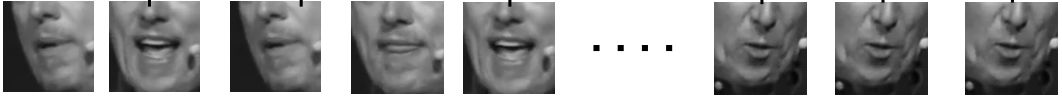
\includegraphics[width=4.35cm,height=0.56cm,keepaspectratio]{avhubert-visual-timesteps.png}};
    \node[font=\tiny,below=0.02cm of visual] {Visual sequence: $v_{1:T}$};
    \node[inner sep=0pt] (audio) at (3.0,0.38)
      {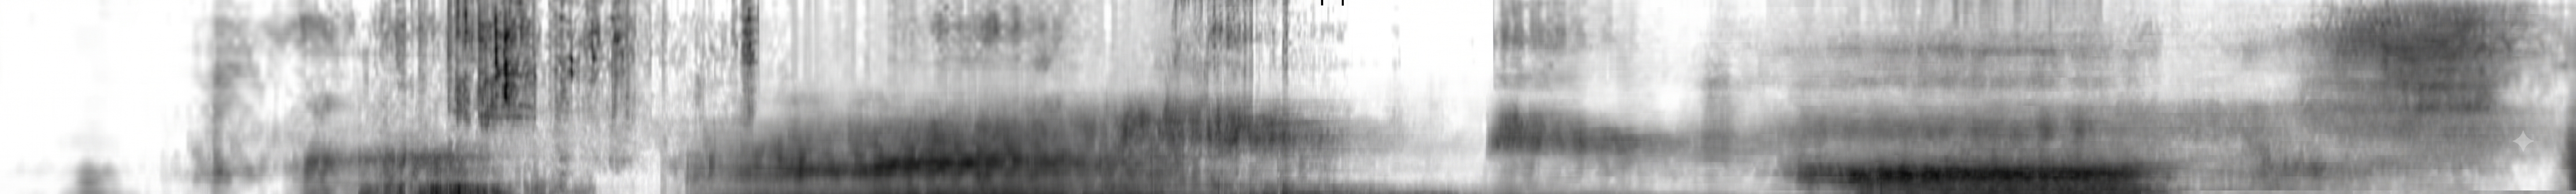
\includegraphics[width=4.35cm,height=0.56cm,keepaspectratio]{avhubert-audio-timesteps_no_mask.png}};
    \node[font=\tiny,below=0.02cm of audio] {Audio sequence: $a_{1:T}$};

    % Shared AV-HuBERT encoder path.
    \node[encoder,text width=3.20cm] (venc) at (-3.0,1.40)
      {\textbf{Visual encoder (ResNet-18)}\\[-0.05cm]$f_t^v=E_v(v_t)$};
    \node[encoder,text width=3.20cm] (aenc) at (3.0,1.40)
      {\textbf{Audio encoder (Linear)}\\[-0.05cm]$f_t^a=E_a(a_t)$};
    \node[fusion,text width=4.35cm] (fusion) at (0,2.48)
      {\textbf{Frame-wise AV fusion}\\[-0.05cm]
       $x_t=[f_t^a;f_t^v]$\\[-0.04cm]
       {\tiny inference keeps both available streams}};
    \node[flow,text width=4.35cm,fill=ClassicBlue!11!white] (transformer) at (0,3.62)
      {\textbf{Transformer context encoder}\\[-0.05cm]
       $H=h_{1:T}=\operatorname{Transformer}(x_{1:T})$};

    % Two complementary decoding scores.
    \node[decoder,text width=3.30cm] (ctc) at (-1.90,4.78)
      {\textbf{CTC prefix scorer}\\[-0.05cm]
       $s_{\mathrm{CTC}}(y_{1:u}\mid H)$\\[-0.04cm]
       {\tiny monotonic alignment}};
    \node[decoder,text width=3.30cm] (attention) at (1.90,4.78)
      {\textbf{Attention decoder}\\[-0.05cm]
       $s_{\mathrm{Att}}(y_{1:u}\mid H)$\\[-0.04cm]
       {\tiny autoregressive context}};
    \node[search,text width=6.25cm] (beam) at (0,5.93)
      {\textbf{Joint beam search}\\[-0.04cm]
       $S(y_{1:u})=\lambda_{\mathrm{dec}}s_{\mathrm{CTC}}
       +(1-\lambda_{\mathrm{dec}})s_{\mathrm{Att}}$};
    \node[output,text width=4.55cm] (transcript) at (0,6.83)
      {\textbf{Vietnamese transcript}\quad
       $\widehat Y=\arg\max_Y S(Y)$};

    % Connectors follow the inference dataflow.
    \draw[arrow] (visual.north) -- (venc.south);
    \draw[arrow] (audio.north) -- (aenc.south);
    \draw[arrow] (venc.north) -- (fusion.south west);
    \draw[arrow] (aenc.north) -- (fusion.south east);
    \draw[arrow] (fusion.north) -- (transformer.south);
    \draw[arrow] (ctc.south |- transformer.north) -- (ctc.south);
    \draw[arrow] (attention.south |- transformer.north) -- (attention.south);
    \draw[arrow] (ctc.north) -- (ctc.north |- beam.south);
    \draw[arrow] (attention.north) -- (attention.north |- beam.south);
    \draw[arrow] (beam.north) -- (transcript.south);
  \end{tikzpicture}

  \note{[Sources] AV-HuBERT.pdf, Section 3.4; ViCocktail Automated Multi-Modal Data Collection for Vietnamese Audio-Visual Speech Recognition.pdf, Section 2.2 and Figure 3; current inference configuration. The diagram reuses the deck's AV-HuBERT encoder visual language and removes training-only masked prediction, pseudo-label generation, and modality dropout.}
\end{frame}


\subsection{Evaluation Metrics}

\begin{frame}{Evaluation Metrics}
  \small
  \begin{columns}[T,onlytextwidth]
    \begin{column}{0.48\textwidth}
      \begin{block}{Word Error Rate (WER)}
        \centering
        \[
          \mathrm{WER}=\frac{S_w+D_w+I_w}{N_w}
        \]
        \raggedright
        \scriptsize
        Measures the proportion of reference word tokens that must be substituted, deleted, or inserted.

        \vspace{0.08cm}
        \textbf{Reference:} hôm nay trời \textcolor{ClassicBlue}{đẹp}\\
        \textbf{Prediction:} hôm nay trời \textcolor{red!75!black}{lạnh}

        \vspace{0.05cm}
        $S_w=1,\ D_w=0,\ I_w=0,\ N_w=4$
        \[
          \mathrm{WER}=\frac{1}{4}=25\%
        \]
      \end{block}
    \end{column}
    \begin{column}{0.48\textwidth}
      \begin{block}{Character Error Rate (CER)}
        \centering
        \[
          \mathrm{CER}=\frac{S_c+D_c+I_c}{N_c}
        \]
        \raggedright
        \scriptsize
        Applies the same edit-distance calculation to characters, revealing smaller spelling and diacritic errors.

        \vspace{0.08cm}
        \textbf{Reference:} t\textcolor{ClassicBlue}{ô}i đang học\\
        \textbf{Prediction:} t\textcolor{red!75!black}{o}i đang học

        \vspace{0.05cm}
        $S_c=1,\ D_c=0,\ I_c=0,\ N_c=12$
        \[
          \mathrm{CER}=\frac{1}{12}\approx 8.3\%
        \]
      \end{block}
    \end{column}
  \end{columns}
  \note{[Sources] src/viavsr/evaluation/error_rates.py; src/viavsr/evaluation/text_normalization.py; tests/evaluation/test_error_rates.py. Spaces are included in the character sequence used by JiWER, so the normalized reference \textit{tôi đang học} contains 12 characters.}
\end{frame}

\subsection{ViCocktail}

\begin{frame}{ViCocktail}
  \small
  \begin{columns}[T,onlytextwidth]
    \begin{column}{0.48\textwidth}
      \begin{block}{Released resource}
        \begin{itemize}
          \item 271 hours, 195,240 utterances, and 2,411 speakers.
          \item Speaker-disjoint test set: 36 speakers, 1,167 utterances.
          \item Automated pipeline for shot detection, face tracking, active-speaker detection, AV sync, lip extraction, and ASR labeling.
          \item First public Vietnamese AVSR dataset with a strong AV-HuBERT baseline.
        \end{itemize}
      \end{block}
    \end{column}
    \begin{column}{0.48\textwidth}
      \begin{block}{What they showed}
        \centering
        \begin{tabular}{lcc}
          \toprule
          Model & Clean & Extreme \\
          \midrule
          Wave2Vec2 & 7.53\% & 70.01\% \\
          AV-HuBERT & 9.40\% & 18.39\% \\
          \bottomrule
        \end{tabular}
        \vspace{0.10cm}

        {\scriptsize Extreme: two interfering speakers at $-5$ dB SNR.}
      \end{block}
      \begin{alertblock}{What they DID NOT show}
        The paper evaluates acoustic interference, but does not directly study partial visual loss within an utterance, such as dropped or unavailable mouth frames.
      \end{alertblock}
    \end{column}
  \end{columns}
  \slidecitation{Source: Nguyen et al., \textit{ViCocktail}, Interspeech 2025, dataset overview and Table 2.}
  \note{[Sources] ViCocktail Automated Multi-Modal Data Collection for Vietnamese Audio-Visual Speech Recognition.pdf, Sections 2-5 and Table 2. The scope-gap statement is our interpretation of the documented construction and evaluation protocol.}
\end{frame}
